\documentclass[twocolumn,11pt]{article}

\textheight 9 in
\voffset -.75 in

\usepackage{amssymb}
\usepackage{amsmath}
\usepackage{graphicx}
\usepackage{epstopdf}
\usepackage{tikz}
\usepackage{fancyhdr}
\usepackage{algpseudocode}
\usepackage[toc,page]{appendix}
\usepackage{url}

\setlength{\parskip}{5pt plus1pt minus1pt}
\setlength{\headheight}{15pt}

\DeclareMathSizes{36}{36}{36}{36}

\title{Train Harder, Smarter:\\Using Graph Theory to Create Route Sugestions}
\author{Forest Trimble\\trimbf@rpi.edu}
\begin{document}

\pagestyle{fancy}
\fancyhead{}
\fancyhead[L]{Forest Trimble}
\fancyhead[R]{Train Harder, Smarter}
\maketitle

\begin{abstract}
  \emph{Cyclists are always in search of the perfect ride on the perfect
  roads. They have criteria like distance and elevation gain to ensure
  that they get in the workout that they want. Unfortunately, in order to
  find this ideal ride manually, it takes a great deal of exploring and
  time, and eventually, one may settle into the habit of using the same
  roads that he/she already knows. We research a way to improve this
  paradigm, and to generate cyclists exactly the route they are looking
  for, without them having to do any work.}
\end{abstract}

\section{Background}

Cycling can be wildly different based on the roads that one takes: On busy
roads with no shoulders, it can be borderline miserable, while few things in
the world are better than spinning down a smoothly paved road with beautiful
vistas of open countryside and no traffic. Unfortunately, cyclists need to
invest massive amounts of time and energy exploring the roads and amassing a
repertoire that they can use. Additionally, it is difficult to satisfy criteria
for training, like an elevation gain and distance, using only that mental
repertoire. This paper chronicles the attempt to unroll a solution for this
problem.

Specifically, a good solution should take as input a distance to travel, a
start point, and, optionally, an elevation gain, and generate a route from the
start point that satisfies the distance and elevation gain within some
$\epsilon$. A fully robust solution would also utilize user data to ensure that
it traverses the most pleasant roads to ride on and avoids the worst.

\section{Tools}

Creating a solution to this problem from scratch would require immense amounts
of time and effort that are simply not available. Fortunately, the larger part
of this problem has already been solved: maps have already been digitized and
parsers for the data format already exist. This section details the various
tools and technologies that the algorithm leverages.

First and foremost, we opted to use the Open Street Map format, which is open
source, fairly robust, and has a very active community that contributes to both
the maps themselves and to various (mostly open-source) software projects that
utilize the format. More information on this format can be found on their
website, openstreetmap.org.

INFO ON OSRM

\section{Algorithm}

The most important part of all of this is how it actually works. The core idea
is that at any point along the route, the engine generates weights for each
different possible direction to take, generates a random number, and picks a
direction according to the random number and the weights. There are several
different ideas that are competing for weight, so we'll break it down into the
individual components first, and then describe the combination at the end.

Additionally, the algorithm requires a few inputs from the user (in addition
to the Open Street Map network of roads):
\begin{itemize}
\item A distance to travel, $d$.
\item A direction in which to head $\phi$.
\item An elevation to gain, $h$.
\item A start point, $x_0$.
\end{itemize}

\subsection{Weight for Distance}

\begin{figure}
  \centering
  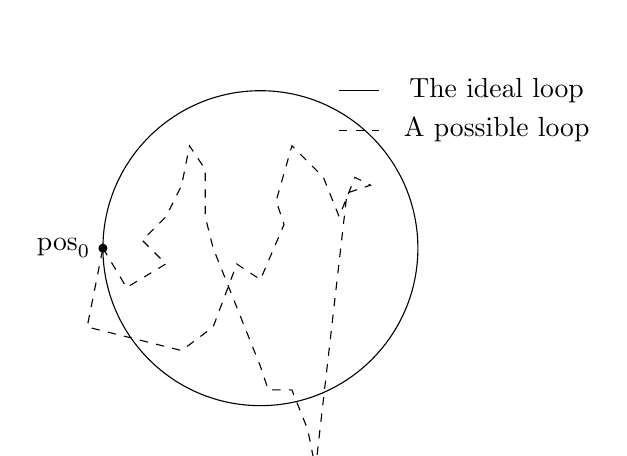
\begin{tikzpicture}
    \node (init) at (-0.5,0) {$\mbox{pos}_0$};
    \filldraw (0,0) circle(0.05);

    \draw (2,0) circle(2);
    \draw[dashed] (0,0) -- (0.3,-.5) -- (0.8,-0.2) -- (0.5,0.1) -- (0.8,0.4) --
    (1.0,0.8) -- (1.1,1.3) -- (1.3,1.0) -- (1.3,0.4) -- (1.4, 0) -- (1.6, -0.5)
    -- (1.8, -1) -- (2.0,-1.5) -- (2.1,-1.8) -- (2.4,-1.8) -- (2.6,-2.3) --
    (2.7,-2.8) -- (3.1,0.7) -- (3.4,0.8) -- (3.2,0.9) -- (3.0,0.4) -- (2.8,0.9)
    -- (2.4,1.3) -- (2.2,0.6) -- (2.3,0.3) -- (2.0,-0.4) -- (1.7, -0.2) --
    (1.4,-1) -- (1.0,-1.3) -- (-0.2,-1) -- (0,0);

    \node (mainleg) at (5,2) {The ideal loop};
    \node (altleg) at (5,1.5) {A possible loop};
    \draw (3,2) -- (3.5,2);
    \draw[dashed] (3,1.5) -- (3.5,1.5);
  \end{tikzpicture}
  \caption{The ideal loop starting at $\mbox{pos}_0$ contrasted with a possible
    actual loop} \label{fig:ideal}
\end{figure}

The first weight is based on distance. The idea is that there is a theoretical,
perfect loop that covers exactly the amount of distance that you would like,
and the algorithm does its best to direct you along that loop. See
Figure~\ref{fig:ideal} for an example of what this might look like.

\begin{figure}
  \centering
  \begin{tikzpicture}
    \node (theta) at (0,4.2) {$\theta$};


    \node (max) at (0.2,3) {2};
    \node (min) at (0.35,1) {0.5};
    \node (avg1) at (-1,2.2) {1};
    \node (avg2) at (1,2.2) {1};

    \draw[thick,<->] (0,0) -- (0,4);
    \draw[thick,<->] (-2,2) -- (2,2);
  \end{tikzpicture}
  \caption{A possible weighted compass} \label{fig:weights}
\end{figure}

In order to direct you along this loop, weights are generated based on
direction. We'll consider the method for finding the optimal direction,
$\theta$, briefly. First, consider how the weights are generated once
that direction is discovered. Basically, there is a weighted compass oriented
along $\theta$, with weights from 0.5 to 2. See Figure~\ref{fig:weights} to
see what we mean. As shown, the weights do not scale linearly, instead, the
weight of any angle, $\tau$, is calculated as follows:
\begin{equation}
  \mbox{WEIGHT} = 2^{1-\frac{2}{\pi}|\theta-\tau|}. \label{eq:weight}
\end{equation}

Now, we consider the method for finding the ideal direction. The idea behind the
direction loop is that if we had an ideal route, it would run exactly along that
path. Then the ideal direction is the one that puts us in the correct location
along that loop. First, consider how the loop is derived. It is a perfect
circle, passing through $x_0$, with a circumfrence of $d$, oriented according to
$\phi$. Note that $d$ and $x_0$ are fairly easy to understand, but the meaning
 of $\phi$ is less obvious. In order to understand what we mean, first consider
the parametric equations for a circle:
\[ x = \cos t \]
\[ y = \sin t \]
These equations generate the unit circle around the origin, something that we
will address later. For now, we are concerned only about what they mean for
$\phi$. Note that without alteration these equations will generate a
west-oriented loop: the circle starts at the rightmost point and proceeds left.
Consider a revised set of equations incorporating $\phi$:
\[ x = \cos (t + \phi) \]
\[ y = \sin (t + \phi). \]
As mentioned already, $\phi = 0$ corresponds to the west-oriented loop, and one
can quickly see that $\phi = \frac{\pi}{2}$ corresponds to the southern loop,
$\phi = \pi$ to the eastern, and $\phi = \frac{3\pi}{2}$ to the northern. That
being said, none of these loops actually start at the proper point; they are
centered around the origin rather than beginning at it. In order to have any
choice of $\phi$ generate a loop that starts at the origin, we can simply zero
out the initial value:
\[ x = \cos (t + \phi) - \cos \phi \]
\[ y = \sin ( t + \phi ) - \sin \phi. \]
This gives a much more obvious representation of our ideal loop, which starts
at (0,0), and traces out a loop according to $\phi$. One thing of interest is
that $\phi$ is exactly $\pi$ plus the compass direction that we would expect.

Once you recall that our distance goal, $d$, is the circumfrence of the loop,
it is easy to see that the radius is $\frac{d}{2\pi}$. We can then adjust our
equation to correspond with our starting point and radius as follows:
\[ x = \frac{d}{2\pi}(\cos ( t + \phi ) - \cos \phi ) + x_0.x \]
\[ y = \frac{d}{2\pi}(\cos ( t + \phi ) - \cos \phi ) + x_0.y \]
Of course, this needs some adjustment to deal with the difference of using
latitude and longitude over a cartesian coordinate system, since latitude
and longitude are not actually coordinates on a 2-d plane, but rather angles
that are made against the center of the Earth. For now, this is sufficient to
get an idea of what is happening, but we'll cover how this will be converted
into a latitude/longitude format in Section~\ref{sec:latlong}.

Until now, we've used $t$ to represent the angle in the parametric equation,
without delving into what it really means. However, we can use a much more
useful expression to represent this angle: $\frac{2\pi}{d}d_i$, where $d_i$ is
the current distance travelled, gives us the
angle in terms of a percentage of the requisite distance travelled. This gives
us the advantage of knowing exactly where in the loop we should be at any
current distance travelled. This also needs to be capped after $d_i \geq d$.
Incorporating this yields the final equations:
\[ x = \frac{d}{2\pi}(\cos (\min(\frac{2\pi}{d}d_i,2\pi) + \phi) - \cos \phi) + x_0.x \]
\[ y = \frac{d}{2\pi}(\sin (\min(\frac{2\pi}{d}d_i,2\pi) + \phi) - \sin \phi)+ x_0.y. \]

\begin{figure}
  \centering
  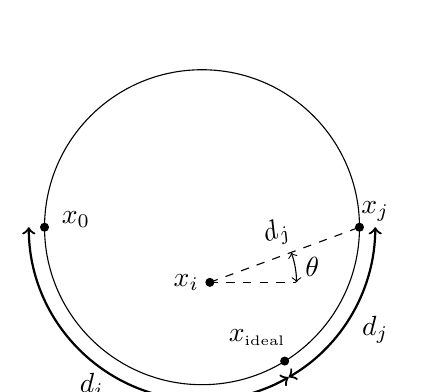
\begin{tikzpicture}
    \draw (2,0) circle(2);
    \filldraw (0,0) circle(0.05);
    \node at (0.4,0.1) {$x_0$};

    \draw[thick,<->] (-0.2,0) arc (180:300:2.2);
    \node at (0.6,-2) {$d_i$};
    \filldraw (3.05,-1.7) circle(0.05);

    \draw[thick,<->] (4.2,0) arc (0:-60:2.2);
    \node at (4.2,-1.3) {$d_j$};

    \filldraw (4,0) circle(0.05);
    \node at (4.2,0.2) {$x_j$};

    \node at (1.8,-0.7) {$x_i$};
    \node at (2.7,-1.4) {$x_{\mbox{{\tiny ideal}}}$};

    \filldraw (2.1,-0.7) circle (0.05);

    \draw[dashed] (2.1,-0.7) -- (4,0) node[above,midway,sloped] {$d_j$};

    \draw[dashed] (2.1,-0.7) -- (3.2,-0.7);
    \draw[<->] (3.2,-0.7) arc(0:20:1.1);
    \node at (3.4,-0.5) {$\theta$};
  \end{tikzpicture}
  \caption{Important values for the algorithm \emph{Note: not to scale}}
  \label{fig:algvals}
\end{figure}

The next step is to utilize these equations to calculate $\theta$. At any point
along the algorithm, we are at some $x_i$, and we have travelled a distance,
$d_i$. Figure~\ref{fig:algvals} should help to understand what exactly the
algorithm is attempting to achieve. The idea is this: if we have travelled some
distance $d_i$, then there is an $x_{\mbox{{\tiny ideal}}}$ on the ``ideal''
loop. The arc between $x_{\mbox{{\tiny ideal}}}$ and $x_0$ will be of length
$d_i$. The algorithm searches for a point $x_j$ such that the arc between
$x_{\mbox{{\tiny ideal}}}$ and $x_j$ will have the \emph{same} distance as the
line between $x_i$ and $x_j$. Fortunately, we have framed the equations for
calculating $x_j$ in terms of the distance travelled along the arc, and the
distance between $x_i$ and $x_j$ can easily be calculated using the pythagorean
theorem. Note that we find $x_j$ as follows:
\begin{align}
  x_j.x = \frac{d}{2\pi} ( & \cos( \frac{ 2 \pi }{ d } ( \min( d, d_i + d_j ) )
                                  + \phi ) \notag \\ & - \cos \phi ) + x_0.x
                                  \label{eq:xjx} \\
  x_j.y = \frac{d}{2\pi} ( & \sin( \frac{ 2 \pi }{ d } ( \min( d, d_i + d_j ) )
                                  + \phi ) \notag \\ & - \sin \phi ) + x_0.y.
                                  \label{eq:xjy}
\end{align}
To satisfy our constraint, we have
\begin{equation}
  d_j = \sqrt{ ( x_j.x - x_i.x )^2 + ( x_j.y - x_i.y )^2 }. \label{eq:dists}
\end{equation}
Obviously, this is a rather difficult equation to truly solve, so we must only
heuristically find a solution. Luckily, we
have a fairly small search space, since $d - d_i > d_j > 0$. On the other hand,
it is not readily apparent how these solutions will behave. We can, however,
be certain that it is continuous, so we can proceed as follows:
\begin{enumerate}
\item Check if the optimal solution would require that we move around the loop
  again. This will happen if
  \[d_i+\sqrt{(x_0.x-x_i.x)^2+(x_0.y-x_i.y)^2} > d.\]
  In this case, we set $x_j = x_0$, and stop searching.
\item \emph{NEEDS MORE WORK}
\end{enumerate}

At this point, we have found $x_j$. From here, calculating $\theta$ is fairly
straightforward:
\begin{align}
  \tan \theta = & \frac{x_j.y - x_i.y}{x_j.x-x_i.x} \notag \\
  \theta = & \tan^{-1} \frac{x_j.y - x_i.y}{x_j.x-x_i.x} \label{eq:theta}
\end{align}

Finally, we have a method for calculating the weights based on distance and
direction! Use \eqref{eq:xjx}, \eqref{eq:xjy}, and \eqref{eq:dists} to find
an $x_j$, and plug into \eqref{eq:theta} to find a $\theta$. Finally, use
$\theta$ in conjunction with \eqref{eq:weight} to assign weights to
directions.

\subsection{Weight for Elevation Gain}

Now that weights have been assigned based on distance and direction, we can
move on to worrying about elevation gain.

FILL IN THIS SECTION

\subsection{Miscellaneous Weights}

There are a few more important characteristics to consider when calculating
weights. Perhaps the easiest of these to deal with are the built in road types
that the Open Street Map format provides. It is easy enough to assign these
priorities based on what a cyclist would reasonably hope to see. Basically,
busy roads get weighted lower than low-traffic roads, but things like
pedestrian walkways and other unridable roads also get high weights.

Another characteristic to consider is whether a road has already been
travelled. Repeatedly riding along the same stretch of road can make a ride
rather boring, so by weighting against this, it can be avoided.

ARE THERE MORE FOR THIS SECTION?

\subsection{Using the Weights Together}

\section{Moving to Three Dimensions} \label{sec:latlong}

\end{document}
